\documentclass[]{book}
\usepackage{lmodern}
\usepackage{amssymb,amsmath}
\usepackage{ifxetex,ifluatex}
\usepackage{fixltx2e} % provides \textsubscript
\ifnum 0\ifxetex 1\fi\ifluatex 1\fi=0 % if pdftex
  \usepackage[T1]{fontenc}
  \usepackage[utf8]{inputenc}
\else % if luatex or xelatex
  \ifxetex
    \usepackage{mathspec}
  \else
    \usepackage{fontspec}
  \fi
  \defaultfontfeatures{Ligatures=TeX,Scale=MatchLowercase}
\fi
% use upquote if available, for straight quotes in verbatim environments
\IfFileExists{upquote.sty}{\usepackage{upquote}}{}
% use microtype if available
\IfFileExists{microtype.sty}{%
\usepackage{microtype}
\UseMicrotypeSet[protrusion]{basicmath} % disable protrusion for tt fonts
}{}
\usepackage{hyperref}
\hypersetup{unicode=true,
            pdftitle={R:从基础到不太基础 - R: from basics to not so basic},
            pdfauthor={Sergio Ibarra-Espinosa},
            pdfborder={0 0 0},
            breaklinks=true}
\urlstyle{same}  % don't use monospace font for urls
\usepackage{natbib}
\bibliographystyle{apalike}
\usepackage{color}
\usepackage{fancyvrb}
\newcommand{\VerbBar}{|}
\newcommand{\VERB}{\Verb[commandchars=\\\{\}]}
\DefineVerbatimEnvironment{Highlighting}{Verbatim}{commandchars=\\\{\}}
% Add ',fontsize=\small' for more characters per line
\usepackage{framed}
\definecolor{shadecolor}{RGB}{248,248,248}
\newenvironment{Shaded}{\begin{snugshade}}{\end{snugshade}}
\newcommand{\AlertTok}[1]{\textcolor[rgb]{0.94,0.16,0.16}{#1}}
\newcommand{\AnnotationTok}[1]{\textcolor[rgb]{0.56,0.35,0.01}{\textbf{\textit{#1}}}}
\newcommand{\AttributeTok}[1]{\textcolor[rgb]{0.77,0.63,0.00}{#1}}
\newcommand{\BaseNTok}[1]{\textcolor[rgb]{0.00,0.00,0.81}{#1}}
\newcommand{\BuiltInTok}[1]{#1}
\newcommand{\CharTok}[1]{\textcolor[rgb]{0.31,0.60,0.02}{#1}}
\newcommand{\CommentTok}[1]{\textcolor[rgb]{0.56,0.35,0.01}{\textit{#1}}}
\newcommand{\CommentVarTok}[1]{\textcolor[rgb]{0.56,0.35,0.01}{\textbf{\textit{#1}}}}
\newcommand{\ConstantTok}[1]{\textcolor[rgb]{0.00,0.00,0.00}{#1}}
\newcommand{\ControlFlowTok}[1]{\textcolor[rgb]{0.13,0.29,0.53}{\textbf{#1}}}
\newcommand{\DataTypeTok}[1]{\textcolor[rgb]{0.13,0.29,0.53}{#1}}
\newcommand{\DecValTok}[1]{\textcolor[rgb]{0.00,0.00,0.81}{#1}}
\newcommand{\DocumentationTok}[1]{\textcolor[rgb]{0.56,0.35,0.01}{\textbf{\textit{#1}}}}
\newcommand{\ErrorTok}[1]{\textcolor[rgb]{0.64,0.00,0.00}{\textbf{#1}}}
\newcommand{\ExtensionTok}[1]{#1}
\newcommand{\FloatTok}[1]{\textcolor[rgb]{0.00,0.00,0.81}{#1}}
\newcommand{\FunctionTok}[1]{\textcolor[rgb]{0.00,0.00,0.00}{#1}}
\newcommand{\ImportTok}[1]{#1}
\newcommand{\InformationTok}[1]{\textcolor[rgb]{0.56,0.35,0.01}{\textbf{\textit{#1}}}}
\newcommand{\KeywordTok}[1]{\textcolor[rgb]{0.13,0.29,0.53}{\textbf{#1}}}
\newcommand{\NormalTok}[1]{#1}
\newcommand{\OperatorTok}[1]{\textcolor[rgb]{0.81,0.36,0.00}{\textbf{#1}}}
\newcommand{\OtherTok}[1]{\textcolor[rgb]{0.56,0.35,0.01}{#1}}
\newcommand{\PreprocessorTok}[1]{\textcolor[rgb]{0.56,0.35,0.01}{\textit{#1}}}
\newcommand{\RegionMarkerTok}[1]{#1}
\newcommand{\SpecialCharTok}[1]{\textcolor[rgb]{0.00,0.00,0.00}{#1}}
\newcommand{\SpecialStringTok}[1]{\textcolor[rgb]{0.31,0.60,0.02}{#1}}
\newcommand{\StringTok}[1]{\textcolor[rgb]{0.31,0.60,0.02}{#1}}
\newcommand{\VariableTok}[1]{\textcolor[rgb]{0.00,0.00,0.00}{#1}}
\newcommand{\VerbatimStringTok}[1]{\textcolor[rgb]{0.31,0.60,0.02}{#1}}
\newcommand{\WarningTok}[1]{\textcolor[rgb]{0.56,0.35,0.01}{\textbf{\textit{#1}}}}
\usepackage{longtable,booktabs}
\usepackage{graphicx,grffile}
\makeatletter
\def\maxwidth{\ifdim\Gin@nat@width>\linewidth\linewidth\else\Gin@nat@width\fi}
\def\maxheight{\ifdim\Gin@nat@height>\textheight\textheight\else\Gin@nat@height\fi}
\makeatother
% Scale images if necessary, so that they will not overflow the page
% margins by default, and it is still possible to overwrite the defaults
% using explicit options in \includegraphics[width, height, ...]{}
\setkeys{Gin}{width=\maxwidth,height=\maxheight,keepaspectratio}
\IfFileExists{parskip.sty}{%
\usepackage{parskip}
}{% else
\setlength{\parindent}{0pt}
\setlength{\parskip}{6pt plus 2pt minus 1pt}
}
\setlength{\emergencystretch}{3em}  % prevent overfull lines
\providecommand{\tightlist}{%
  \setlength{\itemsep}{0pt}\setlength{\parskip}{0pt}}
\setcounter{secnumdepth}{5}
% Redefines (sub)paragraphs to behave more like sections
\ifx\paragraph\undefined\else
\let\oldparagraph\paragraph
\renewcommand{\paragraph}[1]{\oldparagraph{#1}\mbox{}}
\fi
\ifx\subparagraph\undefined\else
\let\oldsubparagraph\subparagraph
\renewcommand{\subparagraph}[1]{\oldsubparagraph{#1}\mbox{}}
\fi

%%% Use protect on footnotes to avoid problems with footnotes in titles
\let\rmarkdownfootnote\footnote%
\def\footnote{\protect\rmarkdownfootnote}

%%% Change title format to be more compact
\usepackage{titling}

% Create subtitle command for use in maketitle
\providecommand{\subtitle}[1]{
  \posttitle{
    \begin{center}\large#1\end{center}
    }
}

\setlength{\droptitle}{-2em}

  \title{R:从基础到不太基础 - R: from basics to not so basic}
    \pretitle{\vspace{\droptitle}\centering\huge}
  \posttitle{\par}
    \author{Sergio Ibarra-Espinosa}
    \preauthor{\centering\large\emph}
  \postauthor{\par}
      \predate{\centering\large\emph}
  \postdate{\par}
    \date{2019-07-07}

\usepackage{booktabs}
\usepackage{amsthm}
\makeatletter
\def\thm@space@setup{%
  \thm@preskip=8pt plus 2pt minus 4pt
  \thm@postskip=\thm@preskip
}
\makeatother

\begin{document}
\maketitle

{
\setcounter{tocdepth}{1}
\tableofcontents
}
\hypertarget{notes}{%
\chapter{Notes}\label{notes}}

CHN:

在本课程中,我将尝试用** CHN \textbf{和英语} ENG **显示中文内容。

ENG:

In this course, I will try to show the content in Chinese with the words \textbf{CHN} and English with \textbf{ENG}

\hypertarget{prerequisites}{%
\chapter{Prerequisites}\label{prerequisites}}

CHN:

本课程专为从未使用过R并依赖Excel丰富多彩功能的人士而设计。
本课程也适用于Linux用户。
如果您使用时空数据,如矢量(shapefiles)和栅格或网格(.Tiff,NetCDF)。
由于我从未见过任何人使用Windows以外的其他人,偶尔也会使用某些Mac,我不希望对/etc/sources.list进行任何更改以保持更新的R或其他任何内容。

ENG:

This course is designed for people who never used R and relies on the colorful functions of Excel.
This course is also for Linux people.
If you work with spatiotemporal data such as vectors (shapefiles) and raster or gridded (.Tiff, NetCDF).
As I never saw anyone using other than Windows and occasionally some Mac, I`m not expecting any change to /etc/sources.list to keep updated R or anything.

I took some examples from R Programming for Data Science (Roger D. Peng, 2016) \url{https://bookdown.org/rdpeng/rprogdatascience/}

\hypertarget{intro}{%
\chapter{Introduction}\label{intro}}

CHN

在开始课程之前,请按照下列步骤操作:

ENG

Before starting the course, follow these steps:

\hypertarget{install-r}{%
\section{Install R}\label{install-r}}

CHN

以这种方式下载R:

1.进入此网页:https://cran.r-project.org/mirrors.html

2.进入任何中国镜子

ENG

Download R in this way:

\begin{enumerate}
\def\labelenumi{\arabic{enumi}.}
\tightlist
\item
  Go into this web page: \url{https://cran.r-project.org/mirrors.html}
\item
  Enter into any Chinese mirror
\end{enumerate}


\includegraphics{fig/01.png}
CHN

例如,让我们进入https://mirrors.tuna.tsinghua.edu.cn/CRAN/
在那里你点击你的系统并下载

ENG

\begin{enumerate}
\def\labelenumi{\arabic{enumi}.}
\setcounter{enumi}{2}
\tightlist
\item
  For instance, lets enter into \url{https://mirrors.tuna.tsinghua.edu.cn/CRAN/}
  There you click on your system and download
\end{enumerate}

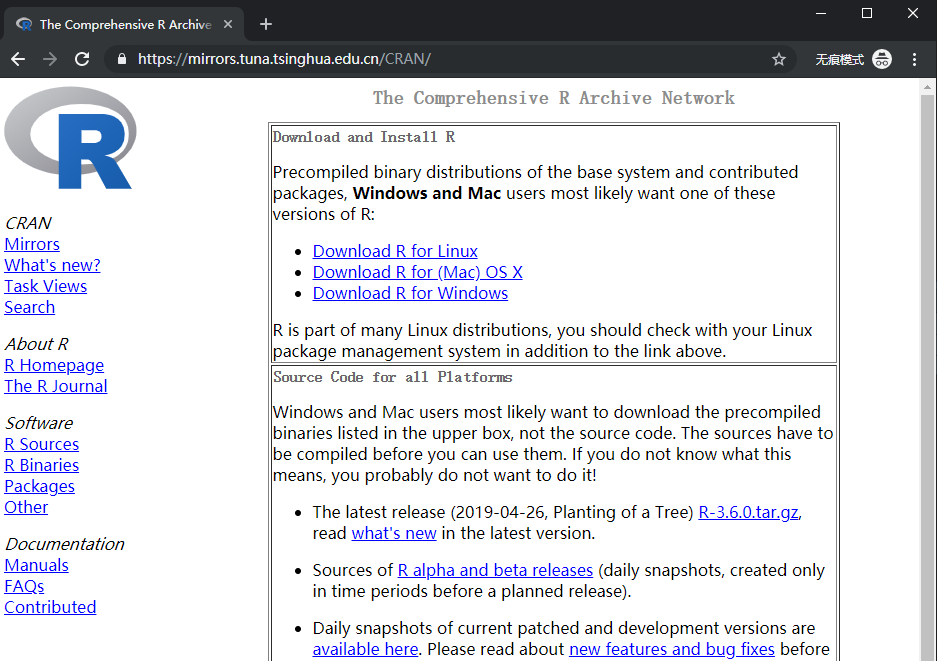
\includegraphics{fig/02.png}

\hypertarget{install-rstudio}{%
\section{Install Rstudio}\label{install-rstudio}}

CHN

进入https://www.rstudio.com,点击Rstudio下载并点击免费下载并安装。

ENG

Go into \url{https://www.rstudio.com}, click on Rstudio Download and click on FREE and download and install.


\includegraphics{fig/03.png}

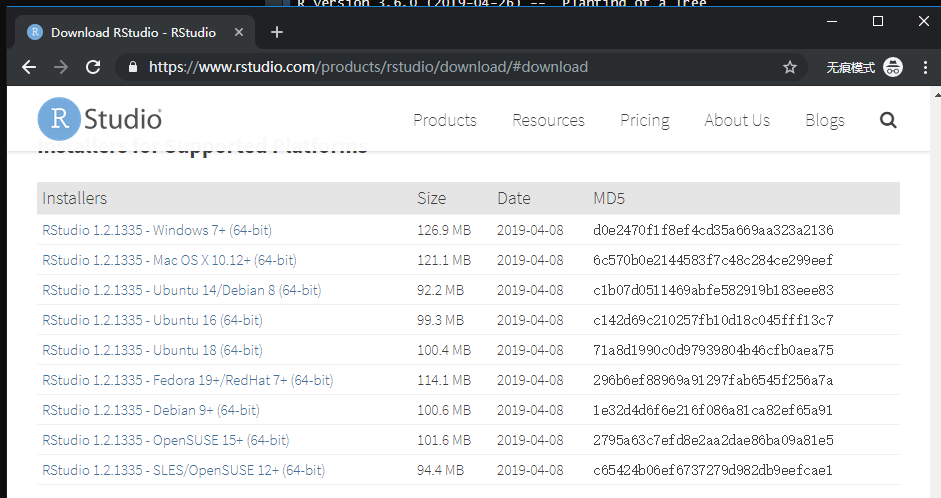
\includegraphics{fig/04.png}

\hypertarget{install-packages}{%
\section{Install packages}\label{install-packages}}

\begin{Shaded}
\begin{Highlighting}[]
\KeywordTok{install.packages}\NormalTok{(}\KeywordTok{c}\NormalTok{(}\StringTok{"ggplot2"}\NormalTok{, }\StringTok{"cptcity"}\NormalTok{, }\StringTok{"sf"}\NormalTok{, }\StringTok{"raster"}\NormalTok{, }\StringTok{"stars"}\NormalTok{, }\StringTok{"data.table"}\NormalTok{,}
                   \StringTok{"readr"}\NormalTok{, }\StringTok{"readxl"}\NormalTok{, }\StringTok{"lubridate"}\NormalTok{))}
\end{Highlighting}
\end{Shaded}

\hypertarget{get-the-data}{%
\section{Get the data}\label{get-the-data}}

\begin{Shaded}
\begin{Highlighting}[]
\KeywordTok{dir.create}\NormalTok{(}\StringTok{"data"}\NormalTok{)}
\KeywordTok{download.file}\NormalTok{(}
  \DataTypeTok{url =} \StringTok{"https://github.com/ibarraespinosa/RIGA/raw/master/data/china_cities_20190413.xlsx"}\NormalTok{, }
  \DataTypeTok{destfile =} \StringTok{"data/china_cities_20190413.xlsx"}\NormalTok{)}
\end{Highlighting}
\end{Shaded}

Download all the files from this link

\url{https://github.com/ibarraespinosa/RIGA/tree/master/data}

\hypertarget{learn-more}{%
\section{Learn more}\label{learn-more}}

Check \url{https://bookdown.org/}

\hypertarget{install-vscode-optional}{%
\section{Install VSCODE (optional)}\label{install-vscode-optional}}

CHN

如果您喜欢Visual Studio(或其他文本编辑器),则可以在其上运行R. 进入此网站并下载并安装

ENG

If you like Visual Studio (or other text editor), you can run R on it. Go into this web and download and install

\url{https://code.visualstudio.com/Download}

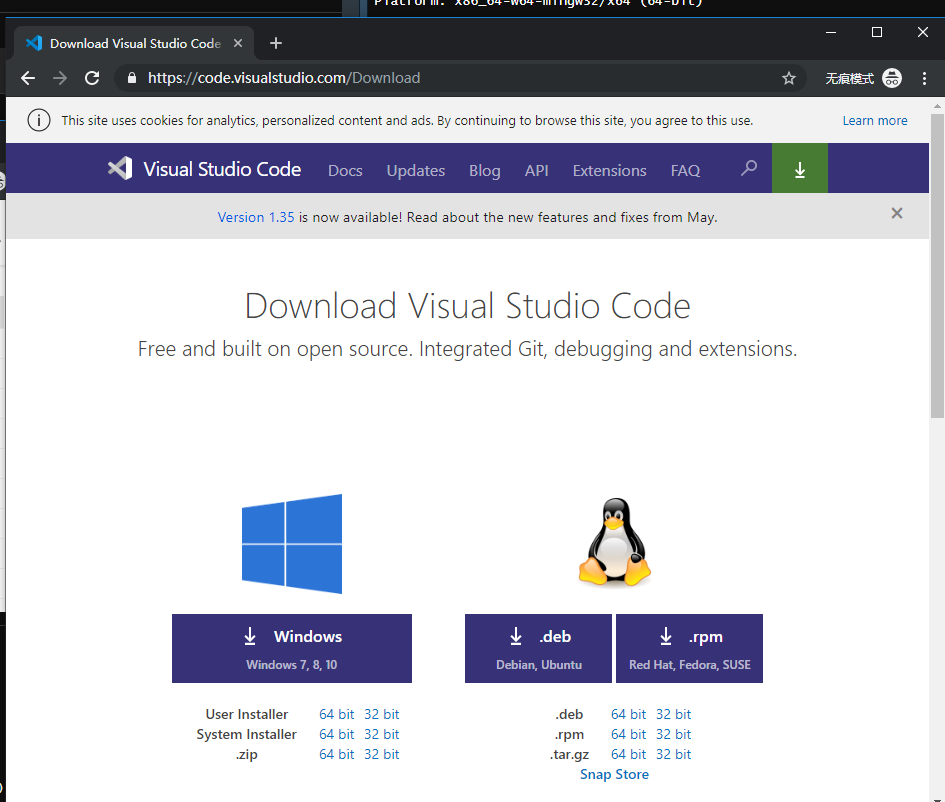
\includegraphics{fig/05.png}

CHN

然后,单击设置,扩展名,r并将路径放在安装R的位置

ENG

Then, click on settings, extensions, r and put the path where you installed R

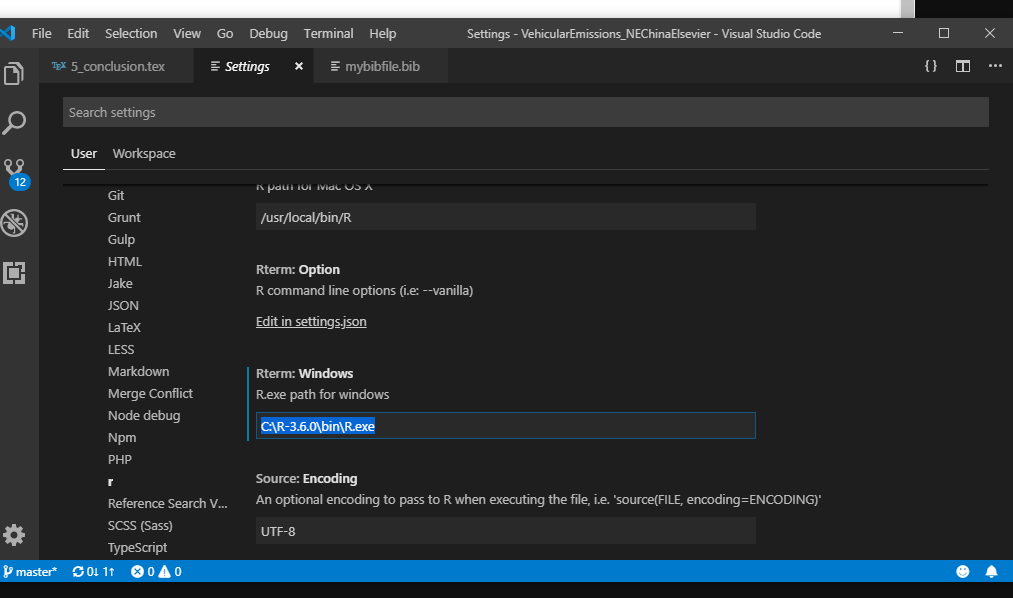
\includegraphics{fig/06.png}

\hypertarget{vectors-and-spreadsheets}{%
\chapter{Vectors and Spreadsheets}\label{vectors-and-spreadsheets}}

\hypertarget{excel---excel-my-old-friend}{%
\section{Excel,我的老朋友 - Excel, my old friend}\label{excel---excel-my-old-friend}}

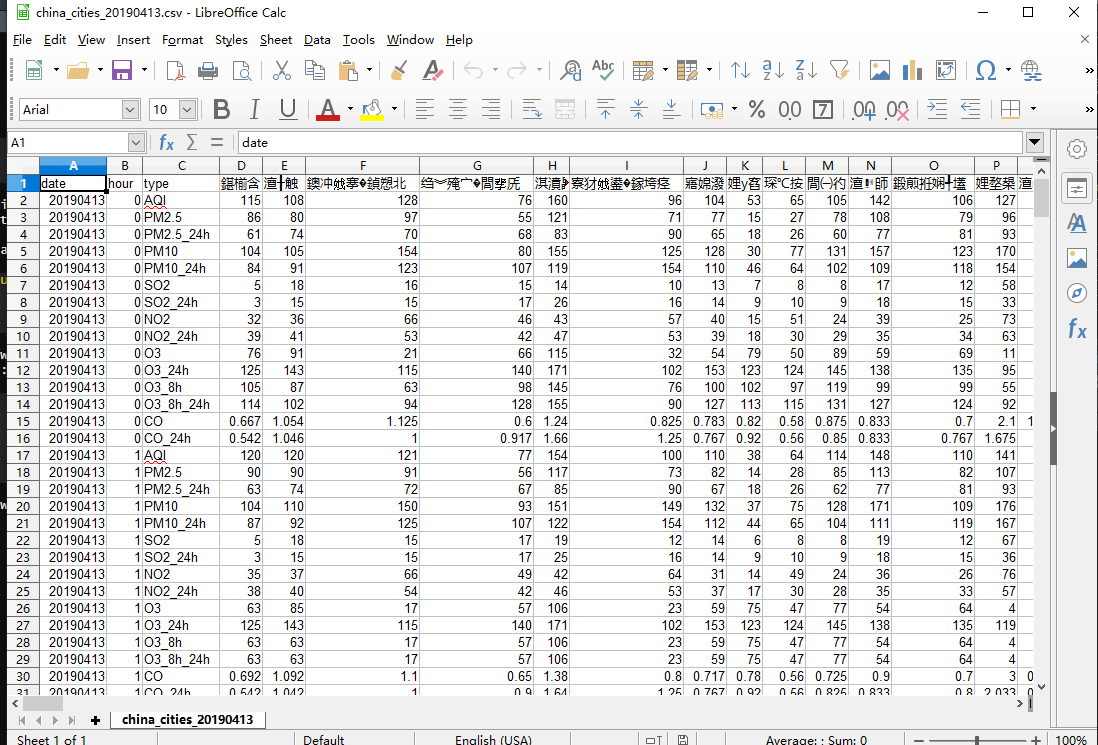
\includegraphics{fig/07.png}
\#\# 输入 - Inputs

\begin{Shaded}
\begin{Highlighting}[]
\NormalTok{x <-}\StringTok{ }\DecValTok{1}
\KeywordTok{print}\NormalTok{(x)}
\NormalTok{x}
\NormalTok{hello <-}\StringTok{ "你好"}
\NormalTok{hello}
\NormalTok{d <-}\StringTok{ }\OtherTok{TRUE}
\NormalTok{d}
\NormalTok{e <-}\StringTok{ }\DecValTok{5} \OperatorTok{+}\StringTok{ }\NormalTok{2i}
\NormalTok{e}
\end{Highlighting}
\end{Shaded}

怎么了? - What is happning?

\hypertarget{objects}{%
\section{对象 - Objects}\label{objects}}

R有5个基本类- R has 5 basic classes

\begin{itemize}
\tightlist
\item
  character
\item
  numeric
\item
  integer
\item
  complex
\item
  logical (TRUE or FALSE) or (T or F)
\end{itemize}

你可以检查这样的类: - You can check the class like this:

\begin{Shaded}
\begin{Highlighting}[]
\NormalTok{a <-}\StringTok{ }\DecValTok{1}\OperatorTok{:}\DecValTok{10}
\NormalTok{a}
\end{Highlighting}
\end{Shaded}

\begin{verbatim}
##  [1]  1  2  3  4  5  6  7  8  9 10
\end{verbatim}

\begin{Shaded}
\begin{Highlighting}[]
\KeywordTok{class}\NormalTok{(a)}
\end{Highlighting}
\end{Shaded}

\begin{verbatim}
## [1] "integer"
\end{verbatim}

\textbf{做(5分钟)}
检查提到的对象的类

\textbf{do (5 min)}
Check the classes of the mentioned objects

\hypertarget{vectors}{%
\section{Vectors}\label{vectors}}

使用函数\texttt{c()}我们创建了将事物连接在一起的向量 - Using the function \texttt{c()}we create vectors concatenating things together

\begin{Shaded}
\begin{Highlighting}[]
\NormalTok{x <-}\StringTok{ }\KeywordTok{c}\NormalTok{(}\FloatTok{0.5}\NormalTok{, }\FloatTok{0.6}\NormalTok{)}
\NormalTok{x}
\NormalTok{x <-}\StringTok{ }\KeywordTok{c}\NormalTok{(}\OtherTok{TRUE}\NormalTok{, }\OtherTok{FALSE}\NormalTok{)}
\NormalTok{x}
\NormalTok{x <-}\StringTok{ }\KeywordTok{c}\NormalTok{(T, F)}
\NormalTok{x}
\NormalTok{x <-}\StringTok{ }\KeywordTok{c}\NormalTok{(}\StringTok{"a"}\NormalTok{, }\StringTok{"b"}\NormalTok{, }\StringTok{"c"}\NormalTok{)}
\NormalTok{x}
\NormalTok{x <-}\StringTok{ }\DecValTok{9}\OperatorTok{:}\DecValTok{29}
\NormalTok{x}
\NormalTok{x <-}\StringTok{ }\KeywordTok{c}\NormalTok{(}\DecValTok{1}\OperatorTok{+}\NormalTok{0i, }\DecValTok{2}\OperatorTok{+}\NormalTok{4i)}
\NormalTok{x}
\end{Highlighting}
\end{Shaded}

\hypertarget{mixing-objects}{%
\section{混合对象 - Mixing objects}\label{mixing-objects}}

如果混合对象会发生什么? - What happens if you mix objects???

\begin{Shaded}
\begin{Highlighting}[]
\NormalTok{x <-}\StringTok{ }\KeywordTok{c}\NormalTok{(}\FloatTok{0.5}\NormalTok{, }\FloatTok{0.6}\NormalTok{)}
\NormalTok{y <-}\StringTok{ }\KeywordTok{c}\NormalTok{(}\StringTok{"a"}\NormalTok{, }\StringTok{"b"}\NormalTok{, }\StringTok{"c"}\NormalTok{)}
\NormalTok{z <-}\StringTok{ }\KeywordTok{c}\NormalTok{(x,y)}
\KeywordTok{class}\NormalTok{(z)}
\end{Highlighting}
\end{Shaded}

\begin{verbatim}
## [1] "character"
\end{verbatim}

\begin{Shaded}
\begin{Highlighting}[]
\NormalTok{y <-}\StringTok{ }\KeywordTok{c}\NormalTok{(}\FloatTok{1.7}\NormalTok{, }\StringTok{"a"}\NormalTok{)}
\NormalTok{y <-}\StringTok{ }\KeywordTok{c}\NormalTok{(}\OtherTok{TRUE}\NormalTok{, }\DecValTok{2}\NormalTok{)}
\NormalTok{y <-}\StringTok{ }\KeywordTok{c}\NormalTok{(}\StringTok{"a"}\NormalTok{, }\OtherTok{TRUE}\NormalTok{)}
\end{Highlighting}
\end{Shaded}

\textbf{做(5分钟)}
检查提到的对象的类

\textbf{do (5 min)}
Check the classes of the mentioned objects

\hypertarget{excel---reading-excel}{%
\subsection{阅读Excel - Reading Excel}\label{excel---reading-excel}}

CHN

有时我们必须使用电子表格(Excel)分析数据。 如果数据很小且分析很简单,则没有问题。 但是什么
如果我们有数百万的混合观察会发生? 使用Excel可能不是一个好主意。

\textbf{做(5分钟)}
打开文件china\_cities\_20190413.xlsx
检查数据
将其导出为.CSV .txt
使用Block Notes打开.CSV文件

ENG

Sometimes we must analize data using spreadsheets (Excel). If the data is small and the analyses is simple, there are no problems. But what
happens if we have millions of mixed observations? Using Excel might be not a good idea.

\textbf{do (5 min)}
Open the file china\_cities\_20190413.xlsx
Check the data
Export it to .CSV or .txt
Open the .CSV file using Block Notes

\begin{Shaded}
\begin{Highlighting}[]
\KeywordTok{library}\NormalTok{(readxl)}
\NormalTok{df <-}\StringTok{ }\KeywordTok{read_xlsx}\NormalTok{(}\StringTok{"data/china_cities_20190413.xlsx"}\NormalTok{)}
\end{Highlighting}
\end{Shaded}

\hypertarget{using-base}{%
\subsection{使用基础 - Using base}\label{using-base}}

\begin{Shaded}
\begin{Highlighting}[]
\NormalTok{df <-}\StringTok{ }\KeywordTok{read.csv}\NormalTok{(}\StringTok{"data/china_cities_20190413.csv"}\NormalTok{, }\DataTypeTok{h =}\NormalTok{ T, )}
\NormalTok{df2 <-}\StringTok{ }\KeywordTok{read.table}\NormalTok{(}\StringTok{"data/china_cities_20190413.txt"}\NormalTok{, }\DataTypeTok{h =}\NormalTok{ T)}
\end{Highlighting}
\end{Shaded}

\hypertarget{data.table---using-data.table}{%
\subsection{使用data.table - Using data.table}\label{data.table---using-data.table}}

data.table比python,julia,spark和dask更快

data.table is faster than python, julia, spark and dask

\textbf{\url{https://h2oai.github.io/db-benchmark/}}

\begin{Shaded}
\begin{Highlighting}[]
\KeywordTok{library}\NormalTok{(data.table)}
\NormalTok{df <-}\StringTok{ }\KeywordTok{fread}\NormalTok{(}\StringTok{"data/china_cities_20190413.csv"}\NormalTok{)}
\end{Highlighting}
\end{Shaded}

\textbf{做(5分钟) - do (5 min)}

\begin{Shaded}
\begin{Highlighting}[]
\KeywordTok{head}\NormalTok{(df)}
\KeywordTok{tail}\NormalTok{(df)}
\NormalTok{df}\OperatorTok{$}\NormalTok{date}
\NormalTok{df[, }\DecValTok{1}\NormalTok{]}
\NormalTok{df}\OperatorTok{$}\NormalTok{hour}
\NormalTok{df[, }\DecValTok{2}\NormalTok{]}
\NormalTok{df}\OperatorTok{$}\NormalTok{date }\OperatorTok{==}\StringTok{ }\NormalTok{df[, }\DecValTok{1}\NormalTok{]}
\NormalTok{df}\OperatorTok{$}\NormalTok{type}
\NormalTok{df}\OperatorTok{$}\NormalTok{鍖椾含}
\end{Highlighting}
\end{Shaded}

现在,检查\textbf{唯一的}值 - Now, check \textbf{unique} values

\begin{Shaded}
\begin{Highlighting}[]
\KeywordTok{unique}\NormalTok{(df}\OperatorTok{$}\NormalTok{type)}
\end{Highlighting}
\end{Shaded}

\begin{verbatim}
##  [1] "AQI"       "PM2.5"     "PM2.5_24h" "PM10"      "PM10_24h" 
##  [6] "SO2"       "SO2_24h"   "NO2"       "NO2_24h"   "O3"       
## [11] "O3_24h"    "O3_8h"     "O3_8h_24h" "CO"        "CO_24h"
\end{verbatim}

CHN

我们可以看到,我们需要过滤我们的数据。 让我们只选择值为'AQI\texttt{的列}type`。
我们只选择日期,时间和第一个中文名称

ENG

As we can see, we need to filter our data. Let us select only the column \texttt{type} with value \texttt{AQI}.
Let us select only the date, time and the first Chinese name

\begin{Shaded}
\begin{Highlighting}[]
\NormalTok{df_aqi <-}\StringTok{ }\NormalTok{df[df}\OperatorTok{$}\NormalTok{type }\OperatorTok{==}\StringTok{ "AQI"}\NormalTok{, }\KeywordTok{c}\NormalTok{(}\StringTok{"date"}\NormalTok{, }\StringTok{"hour"}\NormalTok{, }\StringTok{"鍖椾含"}\NormalTok{)]}
\KeywordTok{head}\NormalTok{(df_aqi)}
\end{Highlighting}
\end{Shaded}

\begin{verbatim}
##        date hour 鍖椾含
## 1: 20190413    0    115
## 2: 20190413    1    120
## 3: 20190413    2    122
## 4: 20190413    3    126
## 5: 20190413    4    130
## 6: 20190413    5    133
\end{verbatim}

CHN

现在,连接日期和小时来创建时间列

ENG

Now, concatenate date and hour to create a time column

\begin{Shaded}
\begin{Highlighting}[]
\KeywordTok{library}\NormalTok{(lubridate)}
\KeywordTok{unique}\NormalTok{(df_aqi}\OperatorTok{$}\NormalTok{hour)}
\end{Highlighting}
\end{Shaded}

\begin{verbatim}
##  [1]  0  1  2  3  4  5  6  7  8  9 10 11 12 13 14 15 16 17 18 19 20 21 22
## [24] 23
\end{verbatim}

\begin{Shaded}
\begin{Highlighting}[]
\NormalTok{df_aqi}\OperatorTok{$}\NormalTok{Time <-}\StringTok{ }\KeywordTok{ymd_h}\NormalTok{(}\KeywordTok{paste}\NormalTok{(df_aqi}\OperatorTok{$}\NormalTok{date, df_aqi}\OperatorTok{$}\NormalTok{hour))}
\end{Highlighting}
\end{Shaded}

现在我们可以策划 - And now we can plot

\hypertarget{plots}{%
\section{Plots}\label{plots}}

\begin{Shaded}
\begin{Highlighting}[]
\KeywordTok{par}\NormalTok{(}\DataTypeTok{mfrow =} \KeywordTok{c}\NormalTok{(}\DecValTok{2}\NormalTok{,}\DecValTok{2}\NormalTok{))}
\KeywordTok{plot}\NormalTok{(}\DataTypeTok{x =}\NormalTok{ df_aqi}\OperatorTok{$}\NormalTok{Time, }\DataTypeTok{y =}\NormalTok{ df_aqi}\OperatorTok{$}\NormalTok{鍖椾含)}
\end{Highlighting}
\end{Shaded}

\begin{verbatim}
## Warning in title(...): 'mbcsToSbcs'里转换'df_aqi$閸栨ぞ鍚�'出错:<e9>代替了
## dot
\end{verbatim}

\begin{verbatim}
## Warning in title(...): 'mbcsToSbcs'里转换'df_aqi$閸栨ぞ鍚�'出错:<8d>代替了
## dot
\end{verbatim}

\begin{verbatim}
## Warning in title(...): 'mbcsToSbcs'里转换'df_aqi$閸栨ぞ鍚�'出错:<96>代替了
## dot
\end{verbatim}

\begin{verbatim}
## Warning in title(...): 'mbcsToSbcs'里转换'df_aqi$閸栨ぞ鍚�'出错:<e6>代替了
## dot
\end{verbatim}

\begin{verbatim}
## Warning in title(...): 'mbcsToSbcs'里转换'df_aqi$閸栨ぞ鍚�'出错:<a4>代替了
## dot
\end{verbatim}

\begin{verbatim}
## Warning in title(...): 'mbcsToSbcs'里转换'df_aqi$閸栨ぞ鍚�'出错:<be>代替了
## dot
\end{verbatim}

\begin{verbatim}
## Warning in title(...): 'mbcsToSbcs'里转换'df_aqi$閸栨ぞ鍚�'出错:<e5>代替了
## dot
\end{verbatim}

\begin{verbatim}
## Warning in title(...): 'mbcsToSbcs'里转换'df_aqi$閸栨ぞ鍚�'出错:<90>代替了
## dot
\end{verbatim}

\begin{verbatim}
## Warning in title(...): 'mbcsToSbcs'里转换'df_aqi$閸栨ぞ鍚�'出错:<ab>代替了
## dot
\end{verbatim}

\begin{Shaded}
\begin{Highlighting}[]
\KeywordTok{plot}\NormalTok{(}\DataTypeTok{x =}\NormalTok{ df_aqi}\OperatorTok{$}\NormalTok{Time, }\DataTypeTok{y =}\NormalTok{ df_aqi}\OperatorTok{$}\NormalTok{鍖椾含, }\DataTypeTok{type =} \StringTok{"l"}\NormalTok{)}
\end{Highlighting}
\end{Shaded}

\begin{verbatim}
## Warning in title(...): 'mbcsToSbcs'里转换'df_aqi$閸栨ぞ鍚�'出错:<e9>代替了
## dot
\end{verbatim}

\begin{verbatim}
## Warning in title(...): 'mbcsToSbcs'里转换'df_aqi$閸栨ぞ鍚�'出错:<8d>代替了
## dot
\end{verbatim}

\begin{verbatim}
## Warning in title(...): 'mbcsToSbcs'里转换'df_aqi$閸栨ぞ鍚�'出错:<96>代替了
## dot
\end{verbatim}

\begin{verbatim}
## Warning in title(...): 'mbcsToSbcs'里转换'df_aqi$閸栨ぞ鍚�'出错:<e6>代替了
## dot
\end{verbatim}

\begin{verbatim}
## Warning in title(...): 'mbcsToSbcs'里转换'df_aqi$閸栨ぞ鍚�'出错:<a4>代替了
## dot
\end{verbatim}

\begin{verbatim}
## Warning in title(...): 'mbcsToSbcs'里转换'df_aqi$閸栨ぞ鍚�'出错:<be>代替了
## dot
\end{verbatim}

\begin{verbatim}
## Warning in title(...): 'mbcsToSbcs'里转换'df_aqi$閸栨ぞ鍚�'出错:<e5>代替了
## dot
\end{verbatim}

\begin{verbatim}
## Warning in title(...): 'mbcsToSbcs'里转换'df_aqi$閸栨ぞ鍚�'出错:<90>代替了
## dot
\end{verbatim}

\begin{verbatim}
## Warning in title(...): 'mbcsToSbcs'里转换'df_aqi$閸栨ぞ鍚�'出错:<ab>代替了
## dot
\end{verbatim}

\begin{Shaded}
\begin{Highlighting}[]
\KeywordTok{plot}\NormalTok{(}\DataTypeTok{x =}\NormalTok{ df_aqi}\OperatorTok{$}\NormalTok{Time, }\DataTypeTok{y =}\NormalTok{ df_aqi}\OperatorTok{$}\NormalTok{鍖椾含, }\DataTypeTok{type =} \StringTok{"b"}\NormalTok{, }\DataTypeTok{pch =} \DecValTok{16}\NormalTok{)}
\end{Highlighting}
\end{Shaded}

\begin{verbatim}
## Warning in title(...): 'mbcsToSbcs'里转换'df_aqi$閸栨ぞ鍚�'出错:<e9>代替了
## dot
\end{verbatim}

\begin{verbatim}
## Warning in title(...): 'mbcsToSbcs'里转换'df_aqi$閸栨ぞ鍚�'出错:<8d>代替了
## dot
\end{verbatim}

\begin{verbatim}
## Warning in title(...): 'mbcsToSbcs'里转换'df_aqi$閸栨ぞ鍚�'出错:<96>代替了
## dot
\end{verbatim}

\begin{verbatim}
## Warning in title(...): 'mbcsToSbcs'里转换'df_aqi$閸栨ぞ鍚�'出错:<e6>代替了
## dot
\end{verbatim}

\begin{verbatim}
## Warning in title(...): 'mbcsToSbcs'里转换'df_aqi$閸栨ぞ鍚�'出错:<a4>代替了
## dot
\end{verbatim}

\begin{verbatim}
## Warning in title(...): 'mbcsToSbcs'里转换'df_aqi$閸栨ぞ鍚�'出错:<be>代替了
## dot
\end{verbatim}

\begin{verbatim}
## Warning in title(...): 'mbcsToSbcs'里转换'df_aqi$閸栨ぞ鍚�'出错:<e5>代替了
## dot
\end{verbatim}

\begin{verbatim}
## Warning in title(...): 'mbcsToSbcs'里转换'df_aqi$閸栨ぞ鍚�'出错:<90>代替了
## dot
\end{verbatim}

\begin{verbatim}
## Warning in title(...): 'mbcsToSbcs'里转换'df_aqi$閸栨ぞ鍚�'出错:<ab>代替了
## dot
\end{verbatim}

\begin{Shaded}
\begin{Highlighting}[]
\KeywordTok{plot}\NormalTok{(}\DataTypeTok{x =}\NormalTok{ df_aqi}\OperatorTok{$}\NormalTok{Time, }\DataTypeTok{y =}\NormalTok{ df_aqi}\OperatorTok{$}\NormalTok{鍖椾含, }\DataTypeTok{type =} \StringTok{"b"}\NormalTok{, }\DataTypeTok{pch =} \DecValTok{16}\NormalTok{,}\DataTypeTok{col =} \StringTok{"red"}\NormalTok{)}
\end{Highlighting}
\end{Shaded}

\begin{verbatim}
## Warning in title(...): 'mbcsToSbcs'里转换'df_aqi$閸栨ぞ鍚�'出错:<e9>代替了
## dot
\end{verbatim}

\begin{verbatim}
## Warning in title(...): 'mbcsToSbcs'里转换'df_aqi$閸栨ぞ鍚�'出错:<8d>代替了
## dot
\end{verbatim}

\begin{verbatim}
## Warning in title(...): 'mbcsToSbcs'里转换'df_aqi$閸栨ぞ鍚�'出错:<96>代替了
## dot
\end{verbatim}

\begin{verbatim}
## Warning in title(...): 'mbcsToSbcs'里转换'df_aqi$閸栨ぞ鍚�'出错:<e6>代替了
## dot
\end{verbatim}

\begin{verbatim}
## Warning in title(...): 'mbcsToSbcs'里转换'df_aqi$閸栨ぞ鍚�'出错:<a4>代替了
## dot
\end{verbatim}

\begin{verbatim}
## Warning in title(...): 'mbcsToSbcs'里转换'df_aqi$閸栨ぞ鍚�'出错:<be>代替了
## dot
\end{verbatim}

\begin{verbatim}
## Warning in title(...): 'mbcsToSbcs'里转换'df_aqi$閸栨ぞ鍚�'出错:<e5>代替了
## dot
\end{verbatim}

\begin{verbatim}
## Warning in title(...): 'mbcsToSbcs'里转换'df_aqi$閸栨ぞ鍚�'出错:<90>代替了
## dot
\end{verbatim}

\begin{verbatim}
## Warning in title(...): 'mbcsToSbcs'里转换'df_aqi$閸栨ぞ鍚�'出错:<ab>代替了
## dot
\end{verbatim}

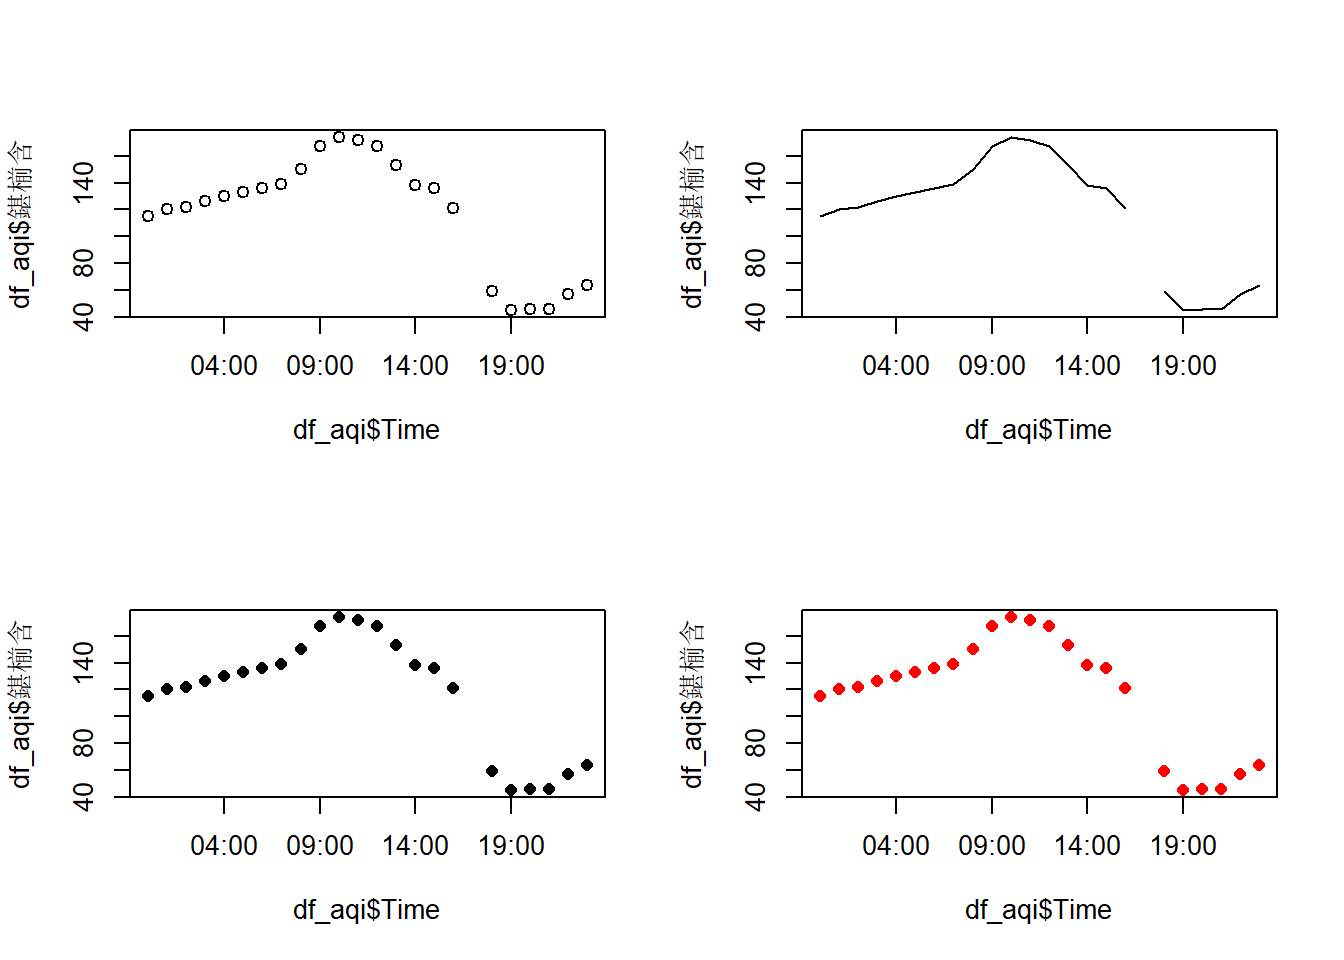
\includegraphics{bookdown-demo_files/figure-latex/unnamed-chunk-23-1.pdf}

\begin{Shaded}
\begin{Highlighting}[]
\KeywordTok{par}\NormalTok{(}\DataTypeTok{mfrow =} \KeywordTok{c}\NormalTok{(}\DecValTok{1}\NormalTok{,}\DecValTok{1}\NormalTok{))}
\end{Highlighting}
\end{Shaded}

Here is a review of existing methods.

You can label chapter and section titles using \texttt{\{\#label\}} after them, e.g., we can reference Chapter \ref{intro}. If you do not manually label them, there will be automatic labels anyway, e.g., Chapter \ref{methods}.

Figures and tables with captions will be placed in \texttt{figure} and \texttt{table} environments, respectively.

\begin{Shaded}
\begin{Highlighting}[]
\KeywordTok{par}\NormalTok{(}\DataTypeTok{mar =} \KeywordTok{c}\NormalTok{(}\DecValTok{4}\NormalTok{, }\DecValTok{4}\NormalTok{, }\FloatTok{.1}\NormalTok{, }\FloatTok{.1}\NormalTok{))}
\KeywordTok{plot}\NormalTok{(pressure, }\DataTypeTok{type =} \StringTok{'b'}\NormalTok{, }\DataTypeTok{pch =} \DecValTok{19}\NormalTok{)}
\end{Highlighting}
\end{Shaded}

\begin{figure}

{\centering 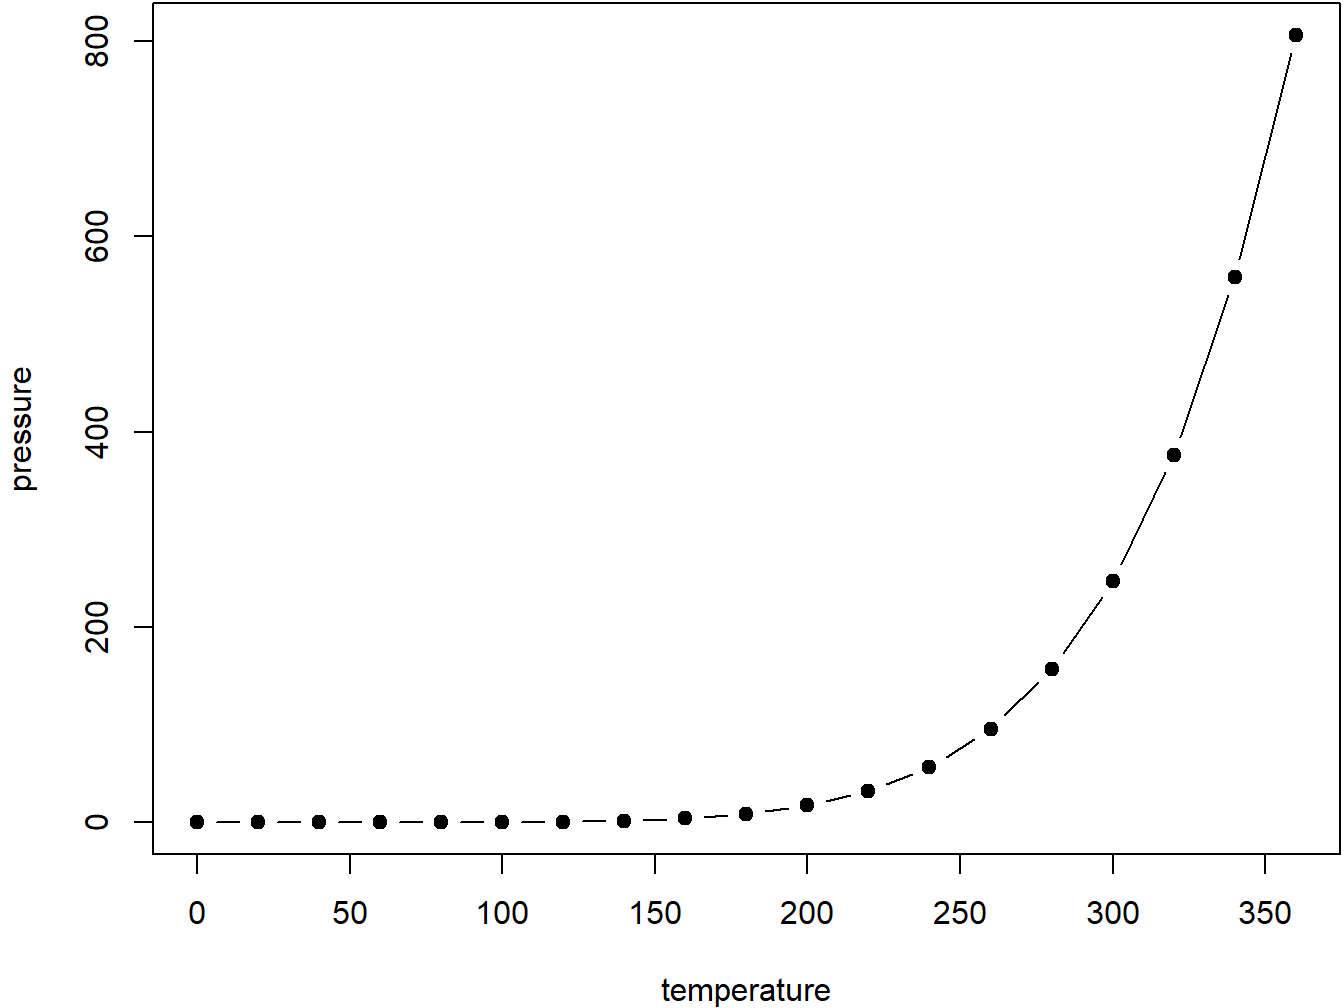
\includegraphics[width=0.8\linewidth]{bookdown-demo_files/figure-latex/nice-fig-1} 

}

\caption{Here is a nice figure!}\label{fig:nice-fig}
\end{figure}

Reference a figure by its code chunk label with the \texttt{fig:} prefix, e.g., see Figure \ref{fig:nice-fig}. Similarly, you can reference tables generated from \texttt{knitr::kable()}, e.g., see Table \ref{tab:nice-tab}.

\begin{Shaded}
\begin{Highlighting}[]
\NormalTok{knitr}\OperatorTok{::}\KeywordTok{kable}\NormalTok{(}
  \KeywordTok{head}\NormalTok{(iris, }\DecValTok{20}\NormalTok{), }\DataTypeTok{caption =} \StringTok{'Here is a nice table!'}\NormalTok{,}
  \DataTypeTok{booktabs =} \OtherTok{TRUE}
\NormalTok{)}
\end{Highlighting}
\end{Shaded}

\begin{table}[t]

\caption{\label{tab:nice-tab}Here is a nice table!}
\centering
\begin{tabular}{rrrrl}
\toprule
Sepal.Length & Sepal.Width & Petal.Length & Petal.Width & Species\\
\midrule
5.1 & 3.5 & 1.4 & 0.2 & setosa\\
4.9 & 3.0 & 1.4 & 0.2 & setosa\\
4.7 & 3.2 & 1.3 & 0.2 & setosa\\
4.6 & 3.1 & 1.5 & 0.2 & setosa\\
5.0 & 3.6 & 1.4 & 0.2 & setosa\\
\addlinespace
5.4 & 3.9 & 1.7 & 0.4 & setosa\\
4.6 & 3.4 & 1.4 & 0.3 & setosa\\
5.0 & 3.4 & 1.5 & 0.2 & setosa\\
4.4 & 2.9 & 1.4 & 0.2 & setosa\\
4.9 & 3.1 & 1.5 & 0.1 & setosa\\
\addlinespace
5.4 & 3.7 & 1.5 & 0.2 & setosa\\
4.8 & 3.4 & 1.6 & 0.2 & setosa\\
4.8 & 3.0 & 1.4 & 0.1 & setosa\\
4.3 & 3.0 & 1.1 & 0.1 & setosa\\
5.8 & 4.0 & 1.2 & 0.2 & setosa\\
\addlinespace
5.7 & 4.4 & 1.5 & 0.4 & setosa\\
5.4 & 3.9 & 1.3 & 0.4 & setosa\\
5.1 & 3.5 & 1.4 & 0.3 & setosa\\
5.7 & 3.8 & 1.7 & 0.3 & setosa\\
5.1 & 3.8 & 1.5 & 0.3 & setosa\\
\bottomrule
\end{tabular}
\end{table}

You can write citations, too. For example, we are using the \textbf{bookdown} package \citep{R-bookdown} in this sample book, which was built on top of R Markdown and \textbf{knitr} \citep{xie2015}.

\hypertarget{methods}{%
\chapter{Methods}\label{methods}}

We describe our methods in this chapter.

\hypertarget{processing-data.frames}{%
\chapter{Processing data.frames}\label{processing-data.frames}}

Some \emph{significant} applications are demonstrated in this chapter.

\hypertarget{example-one}{%
\section{Example one}\label{example-one}}

\hypertarget{example-two}{%
\section{Example two}\label{example-two}}

\hypertarget{spatial-vectors-raster-and-netcdf}{%
\chapter{Spatial vectors, raster and NetCDF}\label{spatial-vectors-raster-and-netcdf}}

Coming soon.

\bibliography{book.bib,packages.bib}


\end{document}
